\chapter{Overleaf \\
\small{\textit{-- Nataly Jimenez, Nicole Valdiviezo, Lakshya Vegiraju}}
\index{Overleaf} 
\index{Chapter!Overleaf}
\label{Chapter::Overleaf}}

\section{Overview}
Overleaf is an online collaborative \LaTeX{} editor that simplifies the writing and publishing of scientific documents. The team deployed it as a Docker container on a DigitalOcean Droplet using free credits from the GitHub Student Developer Pack. This setup provides full control, offline access, and integration with other self-hosted services, such as Bugzilla.

\section{SSH Using Droplet IP}
\begin{minted}{bash}
PS C:\Users\natnj> ssh root@104.248.14.71
root@ubuntu-s-1vcpu-512mb-10gb-nyc3-01:~# snap install docker
\end{minted}

\section{Pull and Run Overleaf Image}
\begin{minted}{bash}
docker run -d -p 8080:80 --name overleaf nginx
http://104.248.14.71:8080/
\end{minted}

\section{Screenshot from Browser}
The following screenshots provide evidence of assignment completion for the Bugzilla section of the project:

\begin{figure}[ht]
    \centering
    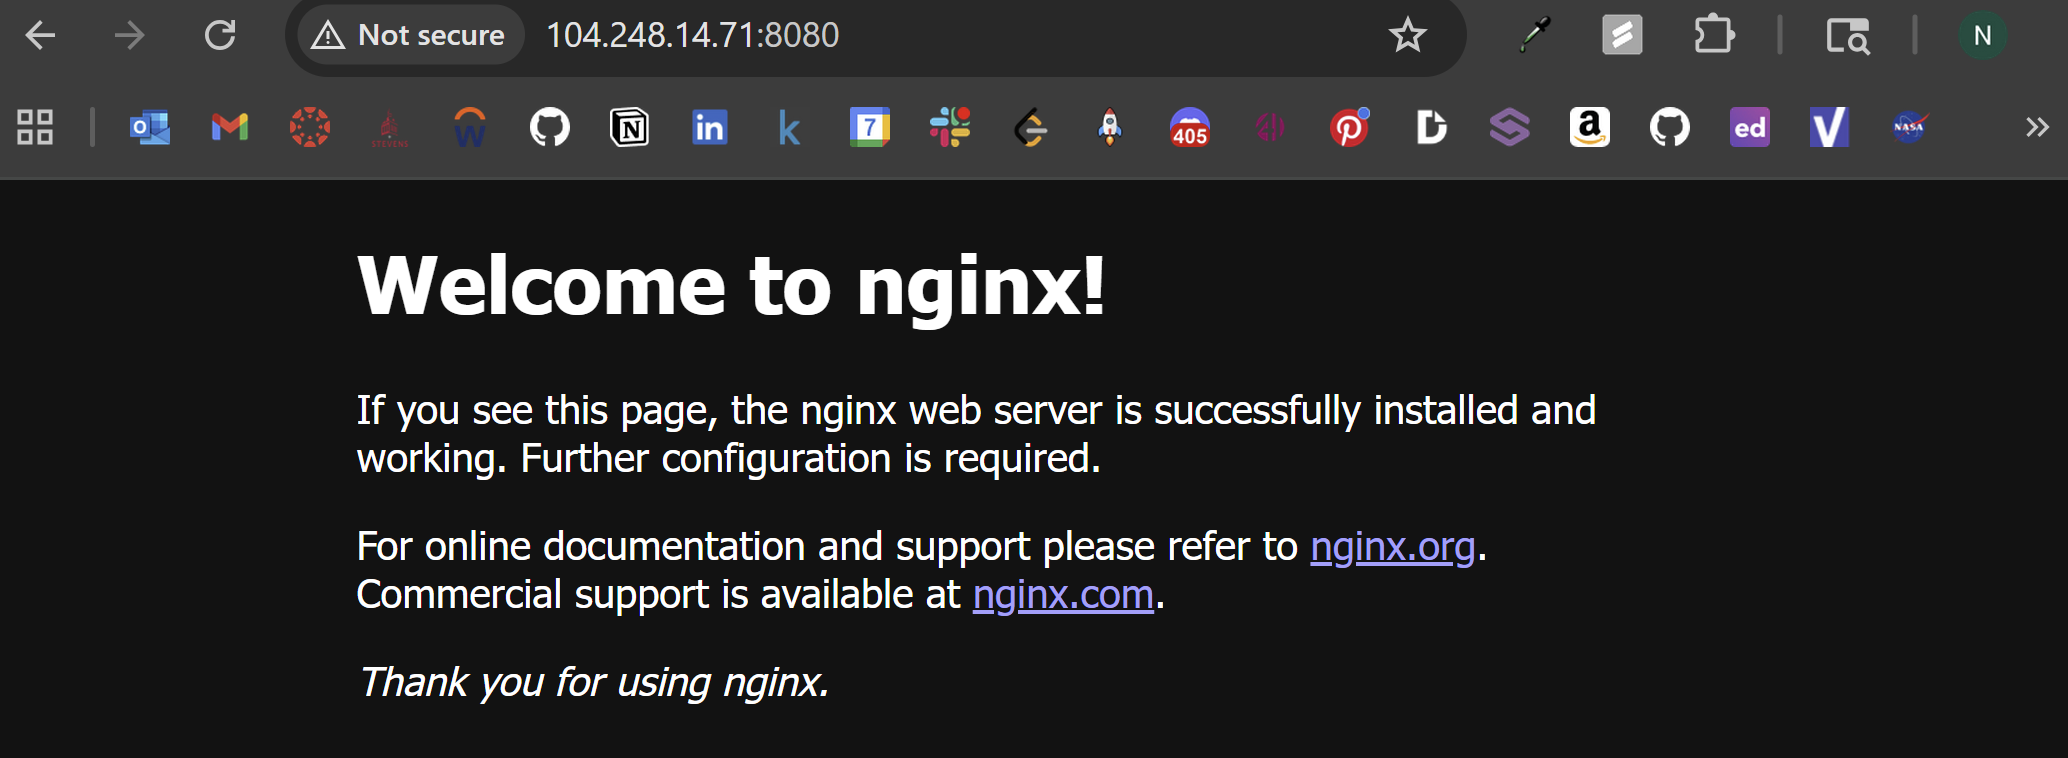
\includegraphics[width=0.6\linewidth]{Book_SSW590_1/eps/Screenshots/Overleaf_6.png}
    \caption{NGINX Page}
    \label{NGINX Page}
\end{figure}
